%% LaTeX2e class for student theses
%% sections/content.tex
%% 
%% Karlsruhe Institute of Technology
%% Institute for Program Structures and Data Organization
%% Chair for Software Design and Quality (SDQ)
%%
%% Dr.-Ing. Erik Burger
%% burger@kit.edu
%%
%% Version 1.1, 2014-11-21



\section{}
\label{sec:}
\citet{mor_mil_PartI} \\
\citet{mor_mil_PartII} \\
\citep{mor_mil_PartIII} \\
\citet{heinze2016large} \\



\chapter{Theoretical Framework}
\label{chap:chap_theo}

\section{Dimensioning of a Helmholtz coil}

\chapter{Materials and Methodology}
\label{chap:chap_mat}

\newacronym{pva}{PVA}{polyvinyl alcohol}
\newacronym{pmma}{PMMA}{polymethyl methacrylate}
\newacronym{ptfe}{PTFE}{polytetrafluorethylen}
\newacronym{fplc}{FPLC}{Fast Protein Liquide Chromatography}
\newacronym{esem}{ESEM}{Environmental scanning electron microscope}

In the first part of this chapter the model setup and implementation using the simulation software COMSOL Multiphysics\textsuperscript{\textregistered}, thereafter referred to as COMSOL, is described.\\
Section \ref{sec:Exp_setup} gives an overview of the experimental setup and execution as well as the analytical methods used. In the last section the mathematical and graphical evaluation is illustrated. 


\section{Model setup/Development}
\label{sec:Model_setup}
The objective of this thesis was the design and implementation of (to establish) an in silico model simulating the retention of magnetic nanoparticles flowing through a magnetizable packed bed. Furthermore parameter studies for various conditions were conducted. In the following the simulation setup including geometry, mesh, boundary conditions and solvers is described.    

\section{Experimental setup / Validation of results}
\label{sec:Exp_setup}
For the validation of the simulation results and a proof of principle of the operational concept several experimental runs were designed. In order to evaluate the retention of a magnetic nanoparticle suspension within a magnetizable packed bed a chromatographic system was used (see Section \ref{subsec:chrom_sys}). The nanoparticle suspension is characterized in Section \ref{subsec:Mag_nanoparticles} and the matrix materials in Section \ref{subsec:Matrix_mat}. Furthermore an overview of the conducted experiments is given in Section \ref{subsec:Exp_Pro}. In Section \ref{subsec:ana_met} the analytical methods and in Section \ref{subsec:Eval} the evaluation methods are discussed.    


\subsection{Magnetic nanoparticle suspension}
\label{subsec:Mag_nanoparticles}
The experiments were conducted with two different types of magnetic nanoparticles. For the experiments in section \ref{subsec:Exp_Pro} a nanoparticle suspension from Chemagen was used. The magnetic nanoparticles from Chemagen consist of a core of magnetite coated with \gls{pva}. A stock solution with a concentration of 73\,g/l was used. In order to minimize aggregation the stock solution was put into an ultrasonic bath for 20 minutes before use. Then the stock solution was diluted 1:100 with 20\,mM sodium phosphate buffer with a pH of 6.5 and filterd through a filter with a pore size of 450\,nm. 
In addition plain nanomag\textsuperscript{\textregistered}-D-spio particles from micromod with mean diameters of 20\,nm and 100\,nm were utilized for the experiments. The micormod nanoparticles are composed of iron oxid domains coated by an unmodified dextran surface. The stock solution with a concentration of 25\,g/l was also diluted 1:100 with a 20\,mM phosphate buffer. In additon a 1:1 mixture of the two nanoparticle sizes was used. In contrast to the Chemagen nanoparticles the micromod particles required no additional ultrasonic treatment and filtration in order to remove aggregates.     

\subsection{Matrix material}
\label{subsec:Matrix_mat}
For the packed bed three different matrix materials were evaluated. In table \ref{table:mat_material} the two magnetizable materials and their corresponding composition are listed. The concentration ranges for the TruForm particles are due to protected confidentiality. %check this! ask for real composition    

\begin{table}[H]
\centering
\caption{Matrix materials and their composition}
\label{table:mat_material}
\begin{tabular}{llllllll}\hline
\multirow{2}{*}{name} & \multirow{2}{*}{charge/lot} & \multirow{2}{*}{producer} & \multicolumn{5}{c}{composition in \%}  \\
& & & Fe & C & Cr & Ni & Mo \\
\hline\hline
SRA-150 & W140401E & H.C. Stark & 83.95 & 0.16 & 12.5  & & \\
TruForm\textsuperscript{TM} 316-3 & 15 & Praxair & 50-75 & & 5-20 &5-20& 1-5\\
\hline
\end{tabular}
\end{table}

The matrix material SRA-150 was already used in preceding experiments by \cite{AndreMaster}. In order to achieve a narrow particle-size distribution the SRA-150 particles were sieved with a mesh size of 25\,\textmu m and 20\,\textmu m respectively. In addition the matrix material TruForm 316-3 was chosen due to its spherical structure and material composition. 
As a negative control \gls{pmma} particles from microParticles GmbH were used. 

\subsection{Column packing}
\label{subsec:col_pack}
As chromatographic column a Omnifit\textsuperscript{\textregistered} BenchMark\textsuperscript{TM} Microbore Chromatography Column was used. The borosilicate glass column has a column length of 10\,mm, a column inside diameter of 3\,mm and a total volume capacity of 0.7\,ml. On both sides of the column endpieces with pre-assembled frits were used to hold back the matrix material. For the experiments with \gls{pmma} and SRA-150 \gls{ptfe} frits with a pore size of 25\,\textmu m were used. In addition punched out polycarbonate filters with a pore size of 2\,\textmu m and an O-ring were added to the inlet and outlet of the column. For the experiments with the TruForm 316-3 matrix material \gls{ptfe} frits with a pore size of 5\,\textmu m were used, no additional filters were necessary. \\   
For the column packing a slurry consisting of the matrix material and either ultra pure water for \gls{pmma} or a 20\,\%Ethanol suspension for SRA-150 and TruForm 316-3 was used. Ethanol was used in order to simplify the packing of the column due to the reduced surface tension. To remove impurities and achieve a narrower particle size distribution the \gls{pmma} matrix material was first mixed with the solvent and left to settel for several minutes. After sedimentation the supernatant was removed and replaced by fresh solvent. This procedure was repeated till the supernatant was a clear fluid. For the other two matrix materials instead of sedimentation a magnet was held to the outside of the falcon to seperate the magnetizable particles from the supernatant.\\   
A CETONI neMESYS syringe pump, controlled by a QmixElements software, was connected to bottom of the column via a tube (see Figure \ref{fig:setup_column}). With this set-up a negative pressure was generated within the column into which the matrix material slurry is drawn from the column inlet. The slurry was added to the column inlet by pipette. Once the column was completely filled the syringe pump was disconnected and the endpiece with the corresponding frit or filter was placed on top of the column. Then the packed bed within the column was compressed with the help of an \gls{fplc}-System. described in Section \ref{subsec:chrom_sys} to eliminate possible cavities. Afterwards the column was again connected to the syring pump and the resulting void at the top filled with new matrix material. This procedure was repeated until no further compression of the matrix material could be observed. The column and the syringe pump are shown in Figure \ref{fig: }
%%%%%%%%%%%%%%%%%%%%Include Figure of setup and column%%%%%%%%%%%%%%%%%%%%%%%%%%%%%%%%%%%%%%%%%%%%%%%%%%%%%%%%%%%%%%%%%%%%%%%%%%%%%%%%%%%%%%%%%%%%%%%%%%%%%%%%%%%%%%


% \begin{figure}[H]
% \centering
% 
% \scalebox{0.30}{\includegraphics{Bioreactor_real.png}}
% \caption{Photobioreactor with 37 light cylinders for the cultivation of microalgae
% \label{fig: Bioreactor_real}
% }
% \end{figure} 
% 
% \begin{figure}[h]
% 		\centering
%           \begin{subfigure}{0.49\textwidth}
%                   \flushleft
%                   \scalebox{0.30}{\includegraphics{Bioreactor_Geometry.png}}
%                   \caption{Lateral view of the photobioreactor}\label{fig:Bioreactor_Geometry}
%           \end{subfigure}
%         \begin{subfigure}{0.49\textwidth}
%                 \flushright
%                 \scalebox{0.32}{\includegraphics{Bioreactor_cross_section.png}}
%                 \caption{Cross section of the photobioreactor}\label{fig:Bioreactor_cross_section}
%         \end{subfigure}
%         \\
%         
%         \caption{Structure of the photobioreactor with 37 light cylinders}
%         \label{fig:Bioreactor}
%   \end{figure}  


\subsection{Chromatographic system}
\label{subsec:chrom_sys}
For the compression of the packed bed within the column and the execution of the retention experiments an Äkta purifier \gls{fplc}-System from GE Healthcare was used. For all connections tubings with an inner diameter of 0.25\,mm (PEEK tubings blue, GE Healtcare Bio-Sciences)were used to achieve a high resolution. The samples were injected via a sample loop with a total volume of 100\,\textmu m. The experiments were conducted with ultra pure water as solvent and a constant flow rate. An inline UV flow cell was used to continuously measure the absorbance of the liquid at a wavelength of 280 nm and to transmit the data to the computer. A conductivity flow cell was used to measure the conductivity of the passing solution. For further analysis the samples were collected by a fraction collector. The regulation of the \gls{fplc}-System and the analysis of the transmitted data was realized by the software Unicorn. The experimental setup is shown in Figure \ref{fig:  }.
%%%%%%%%%%%%%%%Include Figure of ÄKta and Fraction collector%%%%%%%%%%%%%%%%%%%%%

\subsubsection{Chromatographic system with a Helmholtz coil}
\label{subsubsec:helm_coil}
For all experiments a Helmholtz coil was used to create a stable homogeneous magnetic field around the column. The Helmholtz coil consists of an assembly of four coils with the distance D between each other. The whole length of the four coils was based on the length of the column. The other calculated dimensions of the Helmholtz coil can be found in Table \ref{table:Helmholtz_coil}. The Helmholtz coil was constructed so that for a current of 2\,A a magnetic field of 14\,mT was created. The coil was also designed to be used in an ultrasonic bath. The technical drawing for the construction of the used Helmholtz coil is shown in Figure \ref{fig:Helmholtz_coil}\\  
The Helmholtz coil was included in the chromatographic system as shown in Figure \ref{fig: ???}. The coil was connected to a power amplifier (19 Z/500, FG Elektronik) to increase the electrical signal and therefor the magnetic field within the coil. The square wave signals were generated by a function generator (Rigol DG1022, RIGOL Technologies Inc.). The adjustment of the magnetic flux density was achieved by the regulation of the electric current measured with a digital multimeter(MY64, Mastech Group LLC.).   

\begin{table}[H]
\centering
\caption[Dimensions of the Helmholtz coil]{Calculated dimensions of the Helmholtz coil}
\label{table:Helmholtz_coil}
\begin{tabular}{ll}\hline
Parameter &  Value \\
\hline\hline
 number of turns in each coil n & 300 \\
 filling factor F & 0.73\\
 diameter of copper wire $d_{D}$ & 0.70\,mm\\
 coil depth & 10\,cm\\
 distance between coils D & 3.3\,cm \\
 inner radius $R_{i}$ & 3.0\,cm\\ 
 outer radius $R_{a}$ & 4.58\,cm\\
 mean/average radius $R_{m}$ & 3.79\,cm\\
 \hline
\end{tabular}
\end{table}


\begin{figure}[h]
		\centering
          \begin{subfigure}{0.49\textwidth}
                  \flushleft
                  \scalebox{0.40}{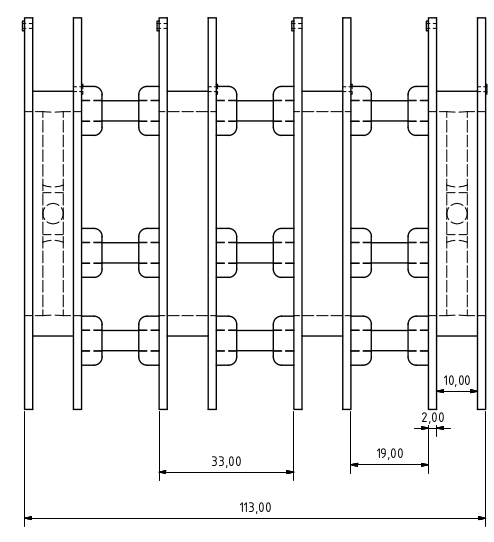
\includegraphics{figures/Helmholtz_Coil_Full.png}}
                  \caption{Side view of the Helmholtz coil}\label{fig:Coil_Full}
          \end{subfigure}
        \begin{subfigure}{0.49\textwidth}
                \flushright
                \scalebox{0.5}{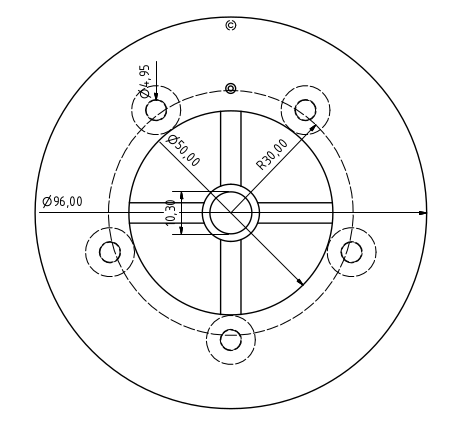
\includegraphics{figures/Helmholtz_Coil_Top.png}}
                \caption{Top view of the Helmholtz coil}\label{fig:Coil_Top}
        \end{subfigure}
        \\
        
        \caption[Technical drawing of the Helmholtz coil]{Technical drawing of the Helmholtz coil with length specifications in mm }
        \label{fig:Helmholtz_coil}
  \end{figure}  

\subsection{Experimental procedures}
\label{subsec:Exp_Pro}
All experiments were programmed and regulated using the control software Unicorn 5.20 (GE Healthcare Life Sciences). Before each injection the column was washed with 2\,ml of ultra pure water to remove remaining nanoparticles from the previous injection. To achieve comparability and reproducibility all experiments were conducted with the same method, except for the fractionation and saturation experiments for which a separate method was created. All experiments were done in triple determination. \\
Before each experiment series the quality of the column packing was controlled. For this purpose a one percent acetone solution was injected and the asymmetry of the  resulting UV peak analyzed. For a packing with \gls{pmma} an asymmetry between 1 and 2 and for a packing with the TruForm particles an asymmetry between 1 and 1.5 was considered tolerable. For deviating asymmetry values the column was emptied and repacked. After each experiment series the column was demagnetized with the help of a degaussing coil (Entmagnetisierer EM-60, MAGNET-PHYSIK Dr. Steingroever GmbH,Köln, Deutschland). Afterwards the column was washed till no significant change in the UV signal was perceived anymore. To clean the filters of the column and reduce the back pressure a change between up- and down-flow was applied while washing when necessary. Once a pressure of 50\,bar was reached the filters were replaced. The blocked filters were regenerated by storing them for 24 hours in oxcalic acid with a concentration of 250\,g/l on a stirrer plate with the lowest heating level.

\subsubsection{Flow rate optimization}
\label{subsubsec:Flow_rate}
In a first step the flow rate was optimized for each matrix material. For this purpose flow rates of 0.1\,ml/min, 0.2\,ml/min and 0.5\,ml/min were tested. The nanoparticle suspension was injected with a volume of 100\,\textmu l and the above mentioned method (see Section \ref{subsec:Exp_Pro}) run with the corresponding flow rates. The resulting UV peaks were analyzed for their asymmetry and reproducibility. Also the comparability with the results form \cite{AndreMaster} was taken into consideration.  

\subsubsection{Retention of magnetic nanoparticle suspension}
\label{subsubsec:Ret_nanopart_method}
The main objective of this experiments was to asses the retention of the magnetic nanoparticles through a magnetized packed bed. The magnetization of the packed bed was achieved by the Helmholtz coil described in Section \ref{subsubsec:helm_coil}. The homogeneous magnetic field within the coil was created by a power amplifier connected to a function generator, which generated an alternating current with a square wave signal. The power amplifier was used to used to change the electric signal and thereby vary the magnetic flux density. For all experiments a flow rate of 0.5\,ml/min and magnetic flux densities between 0\,mT and 17\,mT were used. \\
The magnetic field could be influenced by the variation of the frequency, duty cycle and amplitude. A constant magnetic field was produced by setting the high and low state to the closest values possible. The smallest difference achievable with the used function generator was 4\,mV. Therefor a high level value of 400\,mV and a low level value of 396\,mV was used to approximate a direct current (see Figure \ref{fig:??}). To investigate the impact of an alternating magnetic field the low level was set to -\,400\,mV wereas the high level stayed at 400\,mV. To simulate a magnetic field beeing turned on and off a low level value of 0\,mV was chosen. For the matrix material \gls{pmma} all described variations were applied with the frequencies 100\,mHz and 1000\,mHz . For the matrix material Stark and TruFrom only the constant and on/off fields with frequencies of 100\,mHz, 500\,mHz and 1000\,mHz were tested. The duty cycle, the ratio of the high period to the total period of the square wave, was set to 50\,\% for all experiments. An exception was an experiment with the TruForm particles were the off phase was reduced to 20\,\%.\\ In addition saturation experiments were conducted with the TruForm material. For this the column was first washed with 1\,ml and no magnetic field, next the sample solution was injected and the constant magnetic field turned on. The magnetic field was held till the column was washed with 2\,ml. The cycle was repeated till no further change in the UV peak could be observed. The experiment was conducted twice, once with an used and once with a new filter. A magnetic flux density of 17\,mT was used for the saturation experiments.\\
In order to evaluate the influence of the nanoparticle concentration on the retention behaviour, Chemagen nanoparticel suspension was diluted 1:100, 1:150 and 1:200. The dilutions were tested with TruForm matrix material and a constant magnetic field. The micromod nanoparticle suspensions were also only used for experiments with the TruForm matrix material and a constant magnetic field.\\
For further analysis the third peak of each triple determination was fractionated and collected in 1.5\,ml Eppendorf tubes. A Unicorn method was written to start the fractionation as soon as an increase in the UV signal was detected. As fraction volume 200\,\textmu l was chosen. The fractionation was stopped as soon as the UV signal sank below 0.1\,mAu. 

%%%%%%%%%%%%%%Figure of square wave function%%%%%%%%%%%%%%%%%%%%%%%%%%%%%%%%%%

%%%%%%%%%Tabelle mit Parametern%%%%%%%%%%%%%%%%%%%%%%%%%%%%%%%%%%%%%%%%%%%%%%%%%
 

\subsection{Analytical methods}
\label{subsec:ana_met}
 
 For the characterization of the matrix materials and the nanoparticle suspensions several different analytical methods were used. The particle size distribution was determined either by dynamic light scattering or under the \gls{esem} described in Sections \ref{subsubsec:part_dist_meas} and \ref{subsubsec:ESEM}. The method for the determination of the magnetic properties is described in Section \ref{subsubsec:Mag_char}. For characterization of the magnetic field within the Helmholtz coil a Hall effect sensor is used (see Section \ref{subsubsec:Hall_eff}).   
 
 
\subsubsection{Measurement of particle size distributions}
\label{subsubsec:part_dist_meas}

\subsubsection{Environmental scanning electron microscope}
\label{subsubsec:ESEM}

\subsubsection{Concentration determination of the nanoparticle suspension}
\label{subsubsec:Conc_MF}

\subsubsection{Magnetization determination of the matrix materials and nanoparticle suspension}
\label{subsubsec:Mag_char}

\subsubsection{Analysis of the magnetic flux density}
\label{subsubsec:Hall_eff}
 
\subsection{Evaluation methods}
\label{subsec:Eval}


%%%%%%%%%%%%%%%%%%%%%%%%%%%%%%%%%%%%%%%%%%%%%%%%%%
%%%%%%%%%%%%%%%%%%%%%%%%%%%%%%%%%%%%%%%%%%%%%%%%%%
%%%%%%%%%%%%%%%%%Results%%%%%%%%%%%%%%%%%%%%%%%%%%
%%%%%%%%%%%%%%%%%%%%%%%%%%%%%%%%%%%%%%%%%%%%%%%%%%
%%%%%%%%%%%%%%%%%%%%%%%%%%%%%%%%%%%%%%%%%%%%%%%%%%


\chapter{Results and Discussion}
\label{chap:chap_res}

\section{Simulation results}
\section{Experimental results}


